\chapter{Knee Orthosis Goals}
The knee has been shown to have a non-linear relationship between the flexion and linear movement of the shank with respect to the center of the knee joint. However, few actively actuated orthoses consider this motion, often choosing to consider the knee joint as a pin joint to reduce complexity and the need for multiple different designs for each patient. However, paralysis patients can suffer from serious and significant skin complications if improper fit of their exoskeleton cause rubbing. This thesis aims to develop a knee orthosis that can move with a patient rather than assume a perfect pin joint. I use prior research to determine a desired knee joint relationship. Additionally, the knee should be powered by a high efficiency rotary actuator and be able to support a patient in their rehabilitation efforts.

\section{Design Requirements}
\label{sec:DesignParams}
The following are the design parameters layed out at the beginning of the project:

\subsubsection{Follows the defined knee tibiofemoral trajectory}
The knee joint must be able to follow a tibiofemoral trajectory. As referenced in \cite{KinDynKneeJoint}, human knee joints can be generally defined by a quartic trajectory. This project will use the parameters of a cadaver, which can be seen in \autoref{eq:KneeJointGeometryEquation}. This equation was selected as a goal to prove the effectiveness of the design to follow a desired trajectory. The design of the joint should be easily modifiable to match a patient's individual knee joint. Ideally, all parts except a few should remain the same to increase simplicity and reduce cost of manufacturing.

\begin{equation}
    r(\theta) mm = 1.078\theta^4 - 11.184\theta^3 + 26.524\theta^2 - 0.825\theta
    \label{eq:KneeJointGeometryEquation}
\end{equation}

\subsubsection{Supports the weight of a person}
 Rehabilitation exoskeletons are often designed to only guide the user's body, and therefore do not support the user's body weight. However, to ensure the designed orthosis can be applicable in a multitude of scenarios, a weight requirement was still established. Each joint should be able to support half of the weight of a 85kg human plus a 15kg exoskeleton (total of 100kg) with an additional safety factor.

\subsubsection{Power/Torqe/Speed for walking gaits and sit/stand exercises}

\begin{figure}[ht!]
    \centering
    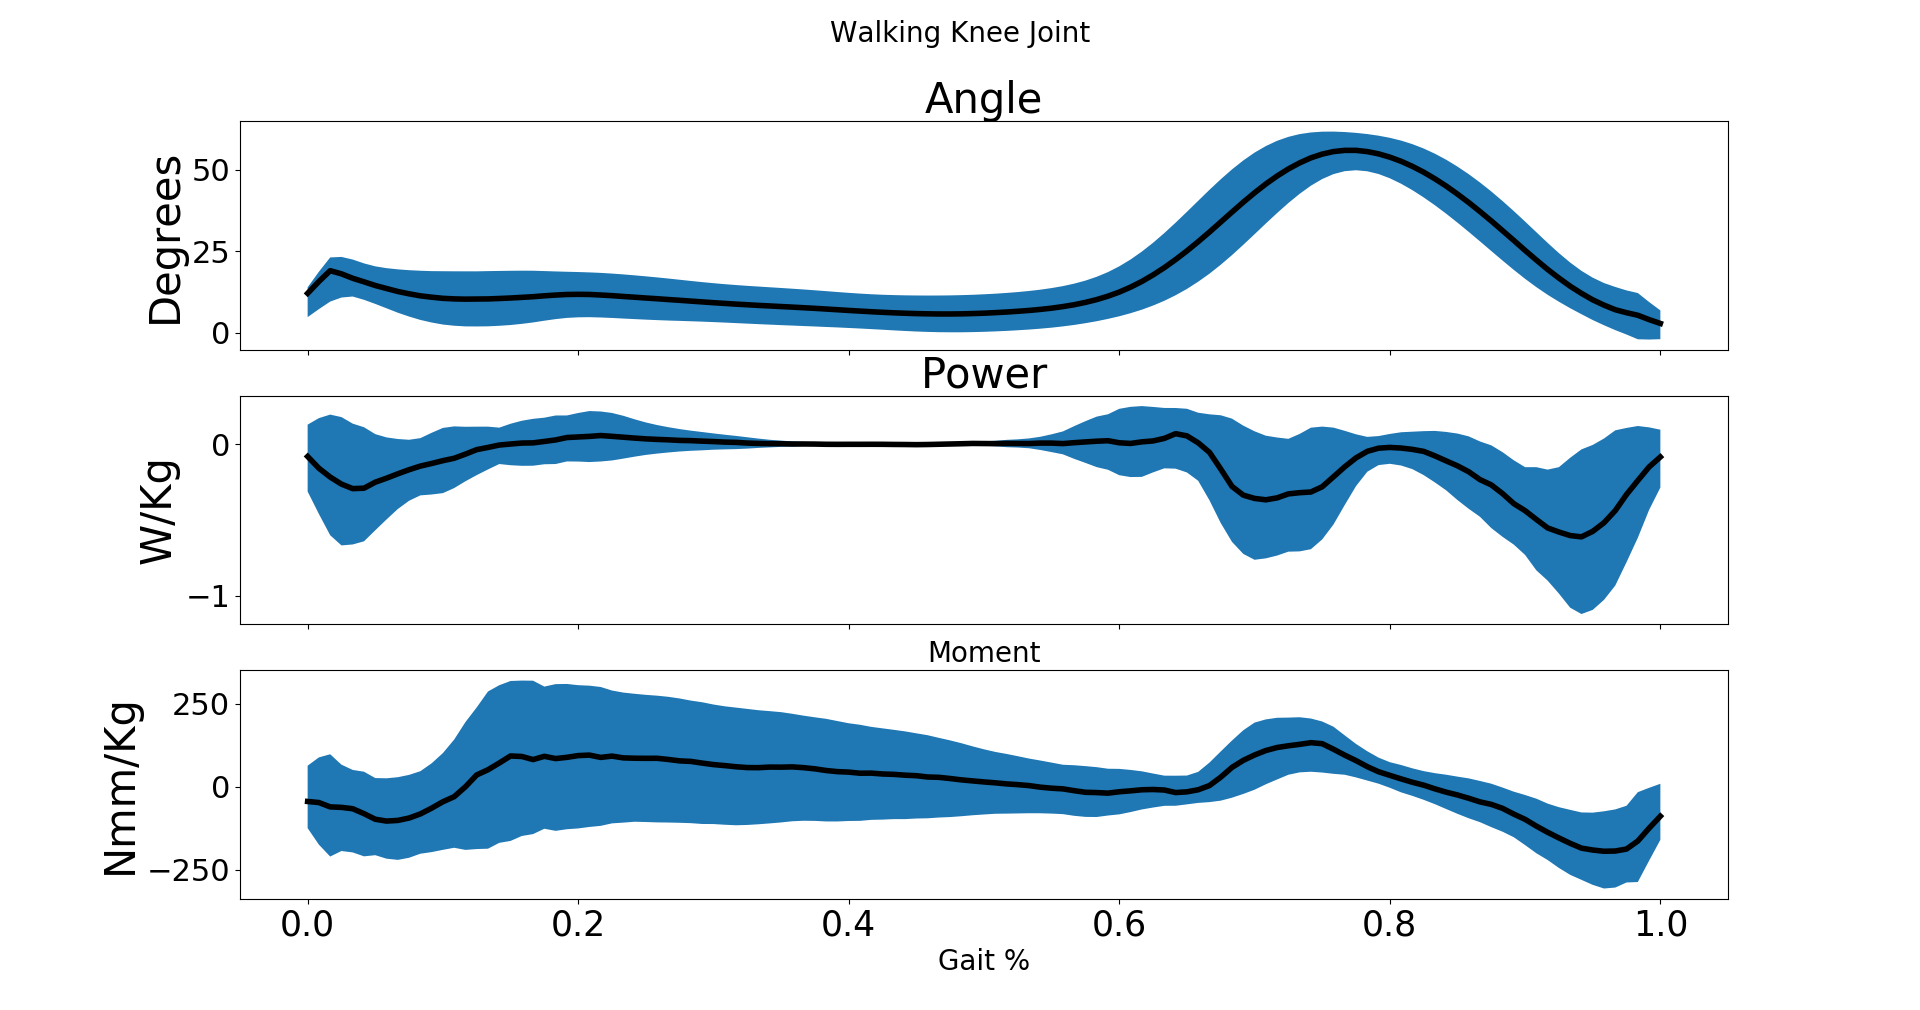
\includegraphics[width=\linewidth]{Figures/Design/WalkingPowerCurveKnee.png}
    \caption{Joint kinematics and dynamics during a walking gait cycle \cite{SpringWrapClutchKnee}}
    \label{fig:WalkingPowerCurve}
\end{figure}

\begin{figure}[ht!]
    \centering
    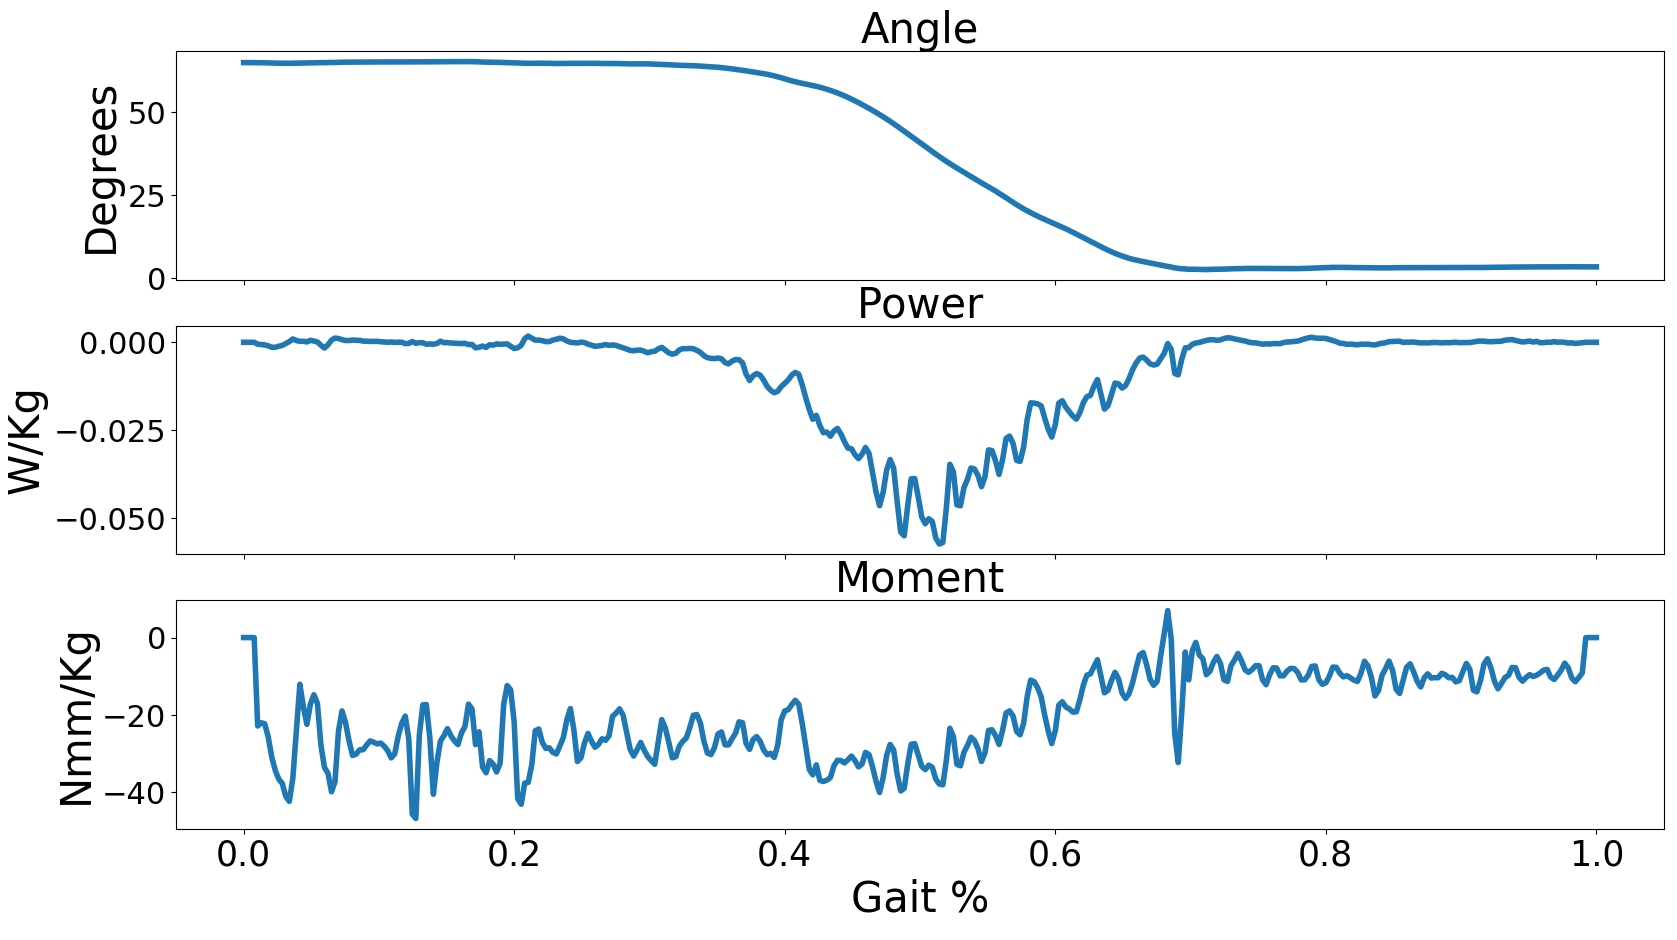
\includegraphics[width=\linewidth]{Figures/Design/SitStandPowerCurveKnee.png}
    \caption{Joint kinematics and dynamics during a standing exercise \cite{SpringWrapClutchKnee}}
    \label{fig:SitStandPowerCurve}
\end{figure}

The knee joint has two rehabilitation requirements to fulfill: walking gaits and sit/stand gaits. Prior research has shown that walking gaits require roughly up to \(0.65 \frac{W}{kg}\) and \(0.25\frac{Nm}{kg}\), (see \autoref{fig:WalkingPowerCurve}), while a sit/stand gait requires roughly up to \(0.5 \frac{W}{kg}\) and \(0.04 \frac{Nm}{kg}\).  Speed requirements are roughly \(120^\circ/sec\) for walking gaits and \(150^\circ/sec\) for sit/stand gaits. Therefore, the designed knee joint for the \(100 kg\) weight specification should be capable of mechanically outputting \(65 W\) and \(25 Nm\) at \(150^\circ/sec\).

\subsubsection{Senses the joint angle}
Sensors must be able to accurately encode the rotational position of the joint. The rationale behind this requirement is for research, debugging, and most importantly accurate and safe position control. Therefore, the joint must be able to read its own position in both passive (non-powered) modes and active (powered) modes. It should also have a minimum accuracy of \(\pm0.5^\circ\) during position control, and be able to maintain position measurement through power cycles (absolute positioning).

\subsubsection{Simple to manufacture and assemble}
The joint must be designed with manufacturing and assembly in mind. All components must be easily sourced and generally available. Any machining requirement must be achievable with common machining techniques.

\subsubsection{Integrates into the WPI LARRE}
This research supports the advancement of the WPI LARRE project introduced in \autoref{sec:larre}. Therefore, the designed joint must be able to integrate into the universal exoskeleton joint connector developed in the LARRE project.